%%%%%%%%%%%%%%%%%%%%%%%%%%%%%%%%%%%%%%%%%%%%%%%%%%%%%%%%%%%%%%%%%%%%%%%%%%%%%%%%
% University of Amsterdam -- Master of AI thesis
% Built on the master_ai_thesis_template (H. Kervadec)
%%%%%%%%%%%%%%%%%%%%%%%%%%%%%%%%%%%%%%%%%%%%%%%%%%%%%%%%%%%%%%%%%%%%%%%%%%%%%%%%

\documentclass{mscaithesis}  % add option [license] to print a CC-BY-NC license page

% Math packages are (on purpose) not included in the class
\usepackage{amssymb}
\usepackage{amsfonts}
\usepackage{amsmath}
\usepackage{amsthm}

\usepackage{natbib}

% Packages required by the thesis content
\usepackage{graphicx}
\usepackage{booktabs}
\usepackage{placeins}
\usepackage[most]{tcolorbox}

% Editing / review helper commands
\newcommand{\red}[1]{{\color{red}{#1}}}
\newcommand{\cs}[1]{\textcolor{orange}{CS: #1}}

%%%%%%%%%%%%%%%%%%%%%%%%%%%%%%%%%%%%%%%%%%%%%%%%%%%%%%%%%%%%%%%%%%%%%%%%%%%%%%%%
% DOCUMENT METADATA
%%%%%%%%%%%%%%%%%%%%%%%%%%%%%%%%%%%%%%%%%%%%%%%%%%%%%%%%%%%%%%%%%%%%%%%%%%%%%%%%

\title{Teacher-Signal Usability in\\ Extreme-Gap Distillation}

\date{2026/06}

\author{Carlos Miguel \textsc{Patiño}}
\studentnumber{15485250}
\period{January -- June 2026}
\credits{36 ECTS}
\examiner{Dr F.~\textsc{Pascoal dos Santos}}
\supervisors{%
        Dr E.~\textsc{Beeching}\\
        Dr K.~\textsc{Rasul}\\
        Dr L.~\textsc{Tunstall}\\
        Prof.\ dr.\ C.G.M.~\textsc{Snoek}%
}

\begin{document}
\maketitle

\frontmatter
        \chapter*{Abstract}
                \begin{adjustwidth}{2cm}{2cm}
                        \begin{abstract}
\red{Provide a short overview and description of your thesis here.}
\end{abstract}

                \end{adjustwidth}

\tableofcontents

\listoffigures

\listoftables

\setlength{\parskip}{5pt}

\chapter{List of Symbols}
        This list of notation can help the reader decipher the thesis:

        \begin{align*}
                x                                       && \text{input prompt;} \\
                y = (y_1, \ldots, y_{L_y})              && \text{output sequence of length $L_y$;} \\
                y_{<n}                                  && \text{prefix $(y_1, \ldots, y_{n-1})$ before token $y_n$;} \\
                V                                       && \text{vocabulary;} \\
                c                                       && \text{privileged context (seen only by the teacher);} \\
                \pi_\theta(\cdot \mid x, y_{<n})        && \text{student policy with parameters $\theta$;} \\
                \pi_T(\cdot \mid x, y_{<n})             && \text{teacher policy;} \\
                \pi_T^{c}                               && \text{teacher policy conditioned on privileged context $c$;} \\
                D_{\mathrm{KL}}(\cdot \,\|\, \cdot)     && \text{Kullback--Leibler divergence;} \\
                k                                       && \text{number of retained top-$k$ tokens;} \\
                S_{T,n}^{k},\; S_{\theta,n}^{k}         && \text{teacher / student top-$k$ token sets at prefix $n$;} \\
                \tau_S                                  && \text{tail bucket grouping all tokens in $V \setminus S$;} \\
                \mathrm{Coverage}_{k}                   && \text{student probability mass inside the teacher top-$k$;} \\
                \mathrm{GapRecovery}                    && \text{fraction of the teacher--student gap recovered.}
        \end{align*}


\chapter{List of Abbreviations}
        \begin{table}[h]
                \centering
                \begin{tabular}{cl}
                                KL      & Kullback--Leibler (divergence) \\
                                FKL     & Forward KL \\
                                RKL     & Reverse KL \\
                                TS-RKL  & Teacher-Support Reverse KL \\
                                SFT     & Supervised fine-tuning \\
                                OPD     & On-policy distillation \\
                                PC      & Privileged context \\
                                CD      & Context distillation \\
                                OOD     & Out-of-distribution \\
                                TRL     & Transformer Reinforcement Learning (library) \\
                                ECTS    & European Credit Transfer System
                \end{tabular}
        \end{table}



\mainmatter
        \include{sections/1-introduction}
        \include{sections/2-related-work}
        \include{sections/3-methods}
        \include{sections/4-experimental-setup}
        \include{sections/5-experiments}
        \chapter{Conclusions}

This thesis set out to study knowledge distillation under extreme teacher--student capacity gaps. The motivation was enabling the most useful setting for distillation: we would like to train very small students because they are cheap and fast to serve, but the most attractive teachers are much larger models because they are more capable. The central question was therefore whether on-policy distillation (OPD), privileged context (PC), and richer token-level teacher feedback could make supervision from very large teachers more usable for much smaller students.

The original hypothesis was that OPD and PC would complement each other. OPD should help because the teacher scores states visited by the student rather than states sampled from a fixed teacher-generated dataset. PC should help because the larger teacher can use additional hidden context when producing its feedback, while the student remains small and unconditioned at inference time. In principle, this combination could exploit the teacher's stronger in-context learning ability without increasing the student's inference cost. We also intended to study whether making rollouts shorter, increasing the number of teacher log probabilities, and using larger teachers would improve the efficiency and performance of the distilled student.

The experiments support the first part of this motivation but not the stronger version of the hypothesis. OPD is consistently better than off-policy SFT in the mathematical reasoning setting we study, which confirms that training on student-generated rollouts is useful under large capacity gaps. However, OPD does not by itself make the largest teacher the best teacher. Scaling from smaller teachers to the 235B teacher does not reliably improve AIME performance, and in several settings the gap recovery rate decreases as the teacher becomes larger. This is the main empirical result of the thesis: under extreme capacity gaps, a more capable teacher does not automatically provide a more learnable training signal.

Privileged context also turned out to be more fragile than expected. A simple PC that tells the teacher about the student and the distillation task already changes downstream performance, but it does not improve the capacity-gap problem and can make teacher scaling worse. A more targeted PC designed to encourage concise mathematical reasoning also fails to beat the simpler alternative of placing the same instruction directly in the system prompt seen by the student. This distinction matters because, in OPD, the student determines the rollout distribution. If the instruction is only hidden in the teacher's scoring context, the student does not generate its rollout under the desired behavior. Direct system prompting changes the states the student visits, and the teacher then provides feedback on those states. In our experiments, this direct conditioning is more effective than trying to distill the hidden context indirectly through teacher logits.

The teacher-assisted privileged-context experiment adds another boundary condition. Giving a 4B scoring teacher access to rollouts from 30B or 235B teachers does not make the signal more usable for the student, and for the 4B student the degradation is especially large. This shows that reducing the apparent capacity gap through a bridge teacher is not sufficient by itself. The bridge teacher must also be capable of using the larger teacher's rollout as helpful context; otherwise the extra context becomes another unusable signal.

The failure analysis shows why this matters. Truncation and substantive reasoning errors dominate the incorrect AIME attempts, with truncation becoming especially severe for the 0.6B student trained with larger teachers. Teacher scaling also increases rollout length substantially, most strongly for the smallest student. This suggests that small students cope with large-teacher feedback by producing longer traces, but the epistemic-word analysis shows that length growth is not simply the same as more explicit reasoning markers. OPD increases epistemic wording relative to the base students, but those markers do not scale with teacher size in the same way rollout length does under brevity interventions. The length explosion therefore appears to be a broader symptom of the capacity gap rather than merely an increase in epistemic self-talk.

The out-of-distribution evaluations show a related tradeoff. The distilled 0.6B student reaches roughly the AIME performance of the same model with reasoning enabled, but its GPQA-Diamond performance declines as the teacher size increases. The 4B student behaves differently: it improves substantially on AIME and remains stable or slightly improves on GPQA-Diamond, although it still does not reach its reasoning-mode AIME reference. This suggests that catastrophic forgetting is not just a side effect of math specialization in general, but depends on the student's capacity to absorb the new reasoning behavior while preserving capabilities outside the training distribution.

The final capacity-effect analysis suggests that the capacity gap is not captured only by the teacher--student size ratio or by the absolute performance gap. The 4B student recovers more of the teacher--student gap than the 0.6B student across the evaluated settings, and the contrast remains visible even when both students are paired with teachers roughly ten times larger and have similar AIME gaps. This suggests that the student's own capacity affects how much of the teacher signal can be turned into improved behavior. In this interpretation, the capacity gap has both a relative component, determined by the distance between teacher and student, and an absolute component, determined by the student's ability to represent and use the supervision it receives.

The top-$K$ experiments reinforce the same conclusion from another direction. Increasing $K$ improves probability mass coverage and should, in principle, give the student a richer approximation of the teacher distribution. In practice, this extra information does not reliably improve performance. The 0.6B student benefits from larger $K$ only when the teacher is the nearby 4B model. With larger teachers, and for the 4B student, increasing $K$ leaves performance unchanged or makes it worse. Higher coverage is therefore not enough because the additional probability mass must also be usable by the student. Under a large capacity gap, richer feedback can become harder rather than easier to learn from.

Taken together, these results shift the conclusion from ``how can we get more signal from the largest teacher?'' to ``how can we make the teacher signal match the student's capacity and rollout distribution?'' The experiments suggest that interventions which directly shape the student's behavior are more reliable than interventions visible only to the teacher. They also show that teacher scale, probability mass coverage, and hidden context are not sufficient proxies for useful supervision. A teacher signal can be more capable, more detailed, and more informed while still being less learnable for the student.

There are also clear limitations. The top-$K$ analysis is limited to $K \in \{1, 10, 50\}$ because transferring teacher log probabilities is expensive at this scale. The experiments also focus on Qwen3 models and mathematical reasoning, so the conclusions should be tested on other model families and tasks before treating them as universal properties of OPD.

Despite these limits, the thesis provides a practical picture of extreme-capacity-gap distillation. OPD is a strong baseline and a better starting point than off-policy distillation, but it does not remove the need to match teacher feedback to student capacity. Privileged context is useful as an experimental tool, but not a general solution by itself. Directly conditioning the student can be more effective than hiding instructions in the teacher. Finally, scaling the amount of teacher information, whether through larger teachers or more top-$K$ log probabilities, can hurt when the student cannot absorb the added complexity, and the smallest student can pay for target-domain gains through out-of-distribution degradation. The systems contribution of the thesis makes these questions easier to study by providing an efficient OPD trainer for large remote teachers, but the empirical lesson is that future methods should focus less on maximizing teacher strength and more on making teacher feedback accessible to the student.


\bibliographystyle{ACM-Reference-Format}
\bibliography{bibliographies/references}

\appendix
        \chapter{Appendix}

\section{OPD vs Off-Policy Methods} \label{sec: exps_off_vs_on}

We compare the three distillation methods that only use feedback from the sampled token at each position. OPD uses the token sampled by the student and scores it under both the student and teacher policies. The two off-policy methods instead use teacher-generated rollouts: SFT treats the sampled token as a hard target, while the soft target objective also includes the teacher log probability for that sampled token.

The results in Figure~\ref{fig: opd_vs_off-policy} show that OPD is stronger than both off-policy methods across all evaluated student--teacher combinations. Among the off-policy methods, SFT consistently performs better than the soft target objective. The soft off-policy objective has worse absolute performance in every setting and also scales worse with teacher size: its gap recovery rate declines more sharply than SFT for both students. These results suggest that, when only the sampled token is available, adding the teacher's probability for a teacher-generated token is not enough to recover the benefit of training on the student's own rollout distribution.

\begin{figure}
    \centering
    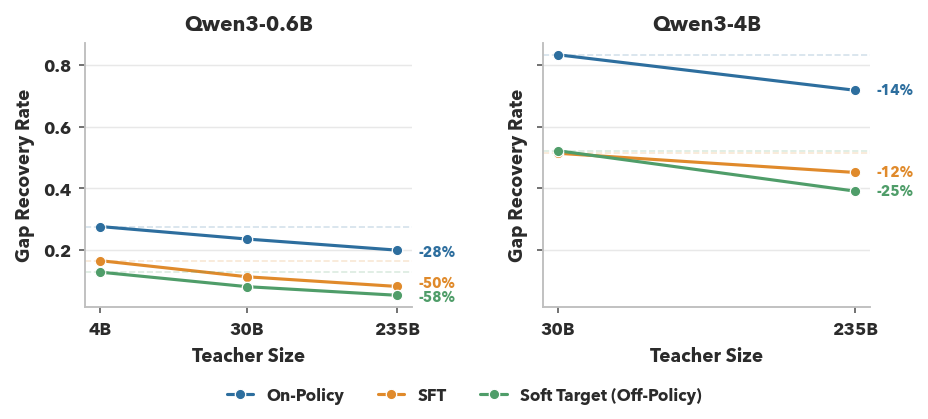
\includegraphics[width=0.9\linewidth]{figures/off_vs_on_policy.png}
    \caption{Gap recovery rate for the three distillation methods that use only the sampled token at each position. OPD performs best for both students across teacher sizes. Among the off-policy methods, SFT is consistently stronger than the soft target objective, which has lower gap recovery in every setting and degrades more when scaling the teacher.}
    \label{fig: opd_vs_off-policy}
\end{figure}

\FloatBarrier

\section{Catastrophic Forgetting in IFEval} \label{sec: app_ifeval_forgettin}

\begin{figure}
    \centering
    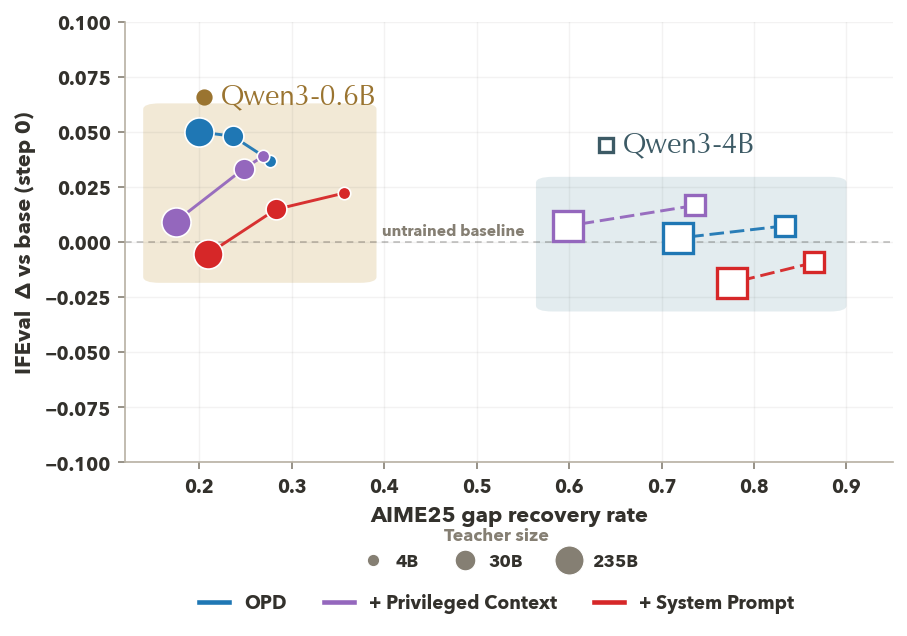
\includegraphics[width=0.9\linewidth]{figures/recovery_aime_vs_ifeval_delta.png}
    \caption{Caption}
    \label{fig: ifeval_reasoning}
\end{figure}

\FloatBarrier

\section{TAID Results}

\begin{figure}
    \centering
    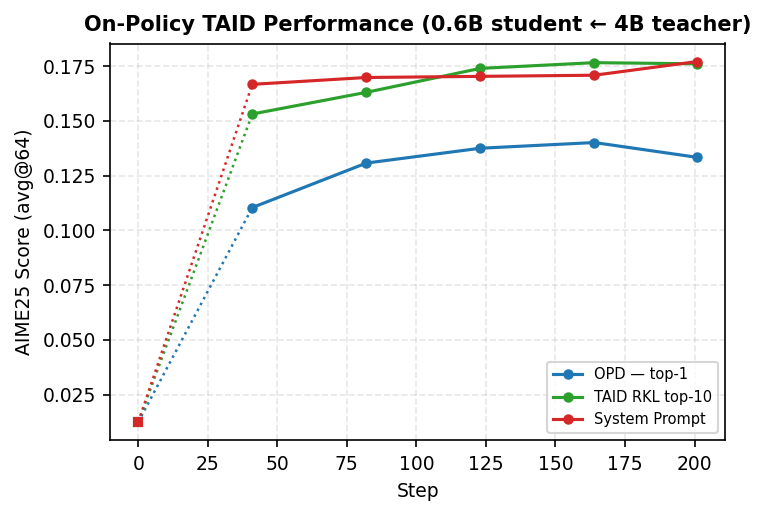
\includegraphics[width=0.9\linewidth]{figures/taid.png}
    \caption{Results for our on-policy implementation of TAID compared to OPD and with the system prompt setup from Section \ref{sec: exps_system_prompt}. The results show that TAID is a promising technique to address the capacity gap because its performance matches our best technique for the 0.6B student and 4B teacher combination.}
    \label{fig:placeholder}
\end{figure}

\FloatBarrier

\section{Hyperparameters} \label{app: hyperparameters}

\begin{table}[htbp]
    \centering
    \small
    \begin{tabular}{ll}
        \toprule
        Hyperparameter & Value \\
        \midrule
        \texttt{temperature} & \texttt{1.0} \\
        \texttt{lmbda} & \texttt{1.0} \\
        \texttt{beta} & \texttt{1.0} \\
        \texttt{max\_completion\_length} & \texttt{4096} \\
        \texttt{num\_generations} & \texttt{4} \\
        \texttt{use\_vllm} & \texttt{true} \\
        \texttt{vllm\_mode} & \texttt{colocate} \\
        \texttt{vllm\_gpu\_memory\_utilization} & \texttt{0.2} \\
        \texttt{bf16} & \texttt{true} \\
        \texttt{gradient\_accumulation\_steps} & \texttt{64} \\
        \texttt{max\_length} & \texttt{8192} \\
        \texttt{per\_device\_train\_batch\_size} & \texttt{1} \\
        \texttt{seed} & \texttt{42} \\
        \texttt{num\_train\_epochs} & \texttt{1} \\
        \texttt{learning\_rate} & \texttt{1e-6} \\
        \texttt{lr\_scheduler\_type} & \texttt{constant\_with\_warmup} \\
        \texttt{warmup\_steps} & \texttt{5} \\
        \bottomrule
    \end{tabular}
    \caption{General hyperparameters used for distillation training. The effective batch size if of 2048 given our 4 nodes with 8 GPUs each. For details on these hyperameters you can refer to \protect\url{https://huggingface.co/docs/trl/distillation_trainer\#trl.experimental.distillation.DistillationConfig}}
    \label{tab:distillation_hyperparameters}
\end{table}

\begin{table}[htbp]
    \centering
    \small
    \begin{tabular}{ll}
        \toprule
        Hyperparameter & Value \\
        \midrule
        \texttt{bf16} & \texttt{true} \\
        \texttt{gradient\_accumulation\_steps} & \texttt{2} \\
        \texttt{per\_device\_train\_batch\_size} & \texttt{4} \\
        \texttt{seed} & \texttt{42} \\
        \texttt{num\_train\_epochs} & \texttt{4} \\
        \texttt{use\_liger\_kernel} & \texttt{true} \\
        \texttt{packing} & \texttt{true} \\
        \texttt{max\_length} & \texttt{8192} \\
        \texttt{learning\_rate} & \texttt{5.0e-05} \\
        \texttt{lr\_scheduler\_type} & \texttt{cosine\_with\_min\_lr} \\
        \texttt{lr\_scheduler\_kwargs.min\_lr\_rate} & \texttt{0.1} \\
        \texttt{warmup\_ratio} & \texttt{0.05} \\
        \bottomrule
    \end{tabular}
    \caption{Hyperparameters used for SFT training. The effective batch size if of 128 given our 4 nodes with 8 GPUs each. For details on these hyperameters you can refer to \protect\url{https://huggingface.co/docs/trl/sft_trainer\#trl.sft.SFTConfig}}
    \label{tab:sft_hyperparameters}
\end{table}

\FloatBarrier

\section{Privileged Information Prompts} \label{app: pc_prompts}

\begin{figure}
    \centering
\begin{tcblisting}{
    enhanced,
    listing only,
    title={Larger-Teacher Rollout Privileged Context},
    fonttitle=\bfseries,
    coltitle=white,
    colback=green!2,
    colframe=green!45!black,
    boxrule=0.6pt,
    arc=1.5mm,
    left=2mm,
    right=2mm,
    top=1.5mm,
    bottom=1.5mm,
    listing options={
        basicstyle=\ttfamily\scriptsize,
        breaklines=true,
        columns=fullflexible,
        keepspaces=true,
        showstringspaces=false,
        escapeinside={(*@}{@*)}
    }
}
(*@\textcolor{blue!70!black}{\texttt{\{prompt\}}}@*)

This is an example for a response to the question:

(*@\textcolor{blue!70!black}{\texttt{\{larger\_teacher\_rollout\}}}@*)
\end{tcblisting}
    \caption{Prompt template used to provide the intermediate teacher with a larger teacher's rollout as privileged context. The student does not see this context when generating its own rollout. The \texttt{prompt} placeholder contains the problem description and the \texttt{larger\_teacher\_rollout} is replaced by the teacher rollout for the prompt.}
    \label{fig: pc_rollout_example}
\end{figure}


\end{document}

%%%%%%%%%%%%%%%%%%%%%%%%%%%%%%%%%%%%%%%%%%%%%%%%%%%%%%%%%%%%%%%%%%%%%%%%%%%%%%%%
%%%%%%%%%%%%%%%%%%%%%%%%%%%%%%%%%%%%%%%%%%%%%%%%%%%%%%%%%%%%%%%%%%%%%%%%%%%%%%%%
